% EXPLAIN THE MODEL
In this section, I develop a model to illustrate the role of dependent values when looking at the trade-off between time consistency and group consistency. I proceed in two steps. First, I describe the baseline model with only one value and show the consequences of an information shock. Then, I replicate the process in a model with two values that are correlated across groups. Thus, I discuss the difference with respect to the single-value model. Lastly, I state the predictions of the model.

\subsection{Single-value model}

Consider an agent with one value $a_t \in \mathbb{R}^2$.\footnote{The agent considers her value with respect to the norm, namely, the average value within the reference population. The reference population can be defined at several levels such as the city, the region, the country, or more broadly, the shared culture. See \citet{Roccas2010Personal} for the importance of the cultural context in the value-behavior relation. See, also, \citet{Bisin2011Economics} for a survey on the economics of cultural transmission and \citet{Rapport2014Social} for a survey on cultural heterogeneity in cultural anthropology. Hence, values are normalized to the population level, so that the mean value in the population is equal to zero.}
The agent belongs to group $s \in \{\underline{s}, \overline{s}\}$ which gather other agents with similar values together.\footnote{They can be seen as close people (including relatives, neighbors, colleagues) since individuals' values are on average correlated within these relationships. But, in a more general setup, they can be seen as peers with whom the agent wants to identify in terms of values.}
The average values within both groups are respectively $\underline{a}$ and $\overline{a}$. 
Suppose the population is sufficiently large to ensure \textit{anonymity}, meaning that any change of value from the agent does not change the distribution, hence, the average values within both groups.
For the remaining of the paper, I set $\overline{a} > 0 > \underline{a}$.

In any period $t$, the agent solves the following maximization program in order to determine her values and the group to which she belongs:
\begin{equation}
    \max_{a_t, s_t} U_t(a_t, s_t) = -\eta_a\frac{\left[a_t-a_{t-1}\right]^2}{2} -\phi_a\frac{\left[a_t-a^\star(s_t)\right]^2}{2},\label{chap3-eq:maxU-1val}
\end{equation}
where $a^\star(s_t)=\{\underline{a}, \overline{a}\}$ is the average value $a$ within her group and $(\eta_a, \phi_a) \in (\mathbb{R}_{+}^\star)^2$ are parameters that account for the relative importance of each utility components.\footnote{These parameters are assumed to be homogeneous within the population, although they might differ across groups of individuals. More extensively, the emergence of heterogeneity in the relative importance of each component would be an interesting point that I leave for future research.} Components of the utility function are expressed in one-dimension Euclidean squared distances. 

The agent seeks to avoid two psychological costs, namely, \textit{time inconsistency} and \textit{group dissonance}. The former implies that the agent prefers when her today’s values are close from her yesterday’s values, thus, she suffers from a utility loss the further her value in period $t$ is from her value in period $t-1$, i.e. $a_t - a_{t-1}$. The literature on social psychology shows that individuals tend to resist changing their attitudes, beliefs, and values through behaviors such as cognitive inertia, or belief perseverance, providing empirical evidence of such a component in agent's utility; see \citet{Kunda1990Case} for a review of biased information processing through which people maintain their beliefs.

The latter psychological cost implies that the agent prefers to hold values that are close to norms within the group to whom she belongs, hence, having a disutility the further her value is from the average value within her group, i.e. $a_t-a^\star(s_t)$. The consistency with the group---to avoid group dissonance---refers to the concept of conformity warp in the social economics literature, meaning that individuals are warped away from their optimal behavior, here values, because they have to conform to the norm; see \citet{Burke2011Social} for a survey on the role of social norms and individual behaviors in presence of norms.

%%%%% OPTIMAL VALUES %%%%%
The optimal value satisfies both the time and group consistencies, hence, it is equal to the weighted average between the agent's value in previous period and the average value in her group. It corresponds to the first-order condition that solves the maximization program \eqref{chap3-eq:maxU-1val}, namely,
\begin{equation}\label{chap3-eq:foc-1val}
    a_t(s_t) =  \frac{\eta_a a_{t-1} + \phi_a a^\star(s_t)}{\eta_a + \phi_a}.
\end{equation}
Thus, the optimal value depends on the group to which the agent decides to belong, hence, to identify.

Suppose that group membership is exogenous, meaning that the agent cannot identify with another group. Thus, she has an initial value $a_0$ and belongs to a group with $a^\star$ as the group-average value. 
The dynamics of the value $a_t$ is derived from equation \eqref{chap3-eq:foc-1val} and correspond to
\begin{equation}\label{chap3-eq:dyn-1val}
    a_t = a^\star + \left(\frac{\eta_a}{\eta_a+\phi_a}\right)^t(a_0-a^\star).
\end{equation}
It is straightforward to show that the value converges toward the average of the group, i.e. $\lim_{t\to+\infty} a_t = a^\star$, at a rate of convergence
\begin{equation*}
    \lim_{t\to+\infty} \frac{\left|a_{t+1}-a^\star\right|}{\left|a_{t}-a^\star\right|} = \frac{\eta_a}{\eta_a+\phi_a} < 1.
\end{equation*}
Thus, leading to Proposition \ref{chap3-prp:converge}. Proof in appendix \ref{chap3-model}.
\begin{proposition}[Value convergence]\label{chap3-prp:converge}
    Any individual converges to the average value within her group and the speed of convergence depends positively on the relative weight of the group consistency (with respect to the time consistency) in the utility function.
\end{proposition}

Let allow the agent to freely choose her group.\footnote{I do not consider any uncertainty in the ability to identify with a group neither any direct cost. Nonetheless, the group consistency corresponds to the psychological, hence indirect, cost of changing group.} She compares both indirect utilities to determine which group she prefers, i.e. $U_t(\overline{s}) - U_t(\underline{s})$. Using the utility function from the maximization problem \eqref{chap3-eq:maxU-1val} along with the optimal value in equation \eqref{chap3-eq:foc-1val}, I obtain
\begin{equation}\label{chap3-eq:uovers-uunders}
    U_t(\overline{s}) - U_t(\underline{s}) = -\gamma_a \left(\left[\overline{a}-a_{t-1}\right]^2 - \left[a_{t-1}-\underline{a}\right]^2\right),
\end{equation}
where $\gamma_a \equiv \frac{\eta_a\phi_a}{2(\eta_a+\phi_a)} >0$. The agent weakly prefers her group to the other as long as her indirect utility in this group is greater or equal to the one she would get in the other.

%%%%% VALUE CONVERGENCE IN SINGLE-VALUE MODEL %%%%%
Let $\widetilde{a}$ be the \textit{indifference value} which is defined as the threshold value in $t-1$ such that the agent is indifferent between both groups in period $t$, i.e. $U_t(\overline{s}) - U_t(\underline{s}) = 0$.
Using equation \eqref{chap3-eq:uovers-uunders}, the indifference value is $\widetilde{a} = \widehat{a}$, where $\widehat{a} \equiv (\overline{a}+\underline{a})/2$ is the \textit{midpoint value}.
The midpoint value refers to the middle of the distance between the average values in both groups and represents the frontier between both groups.\footnote{The anonymity of the agent ensures that the frontier is exogenous.}

Figure \ref{chap3-fig:theory-choice-a} illustrates the indifference value and group membership.
\begin{figure}[!tb]
    \centering
    \caption{Indifference value and group membership}
    \label{chap3-fig:theory-choice-a}
    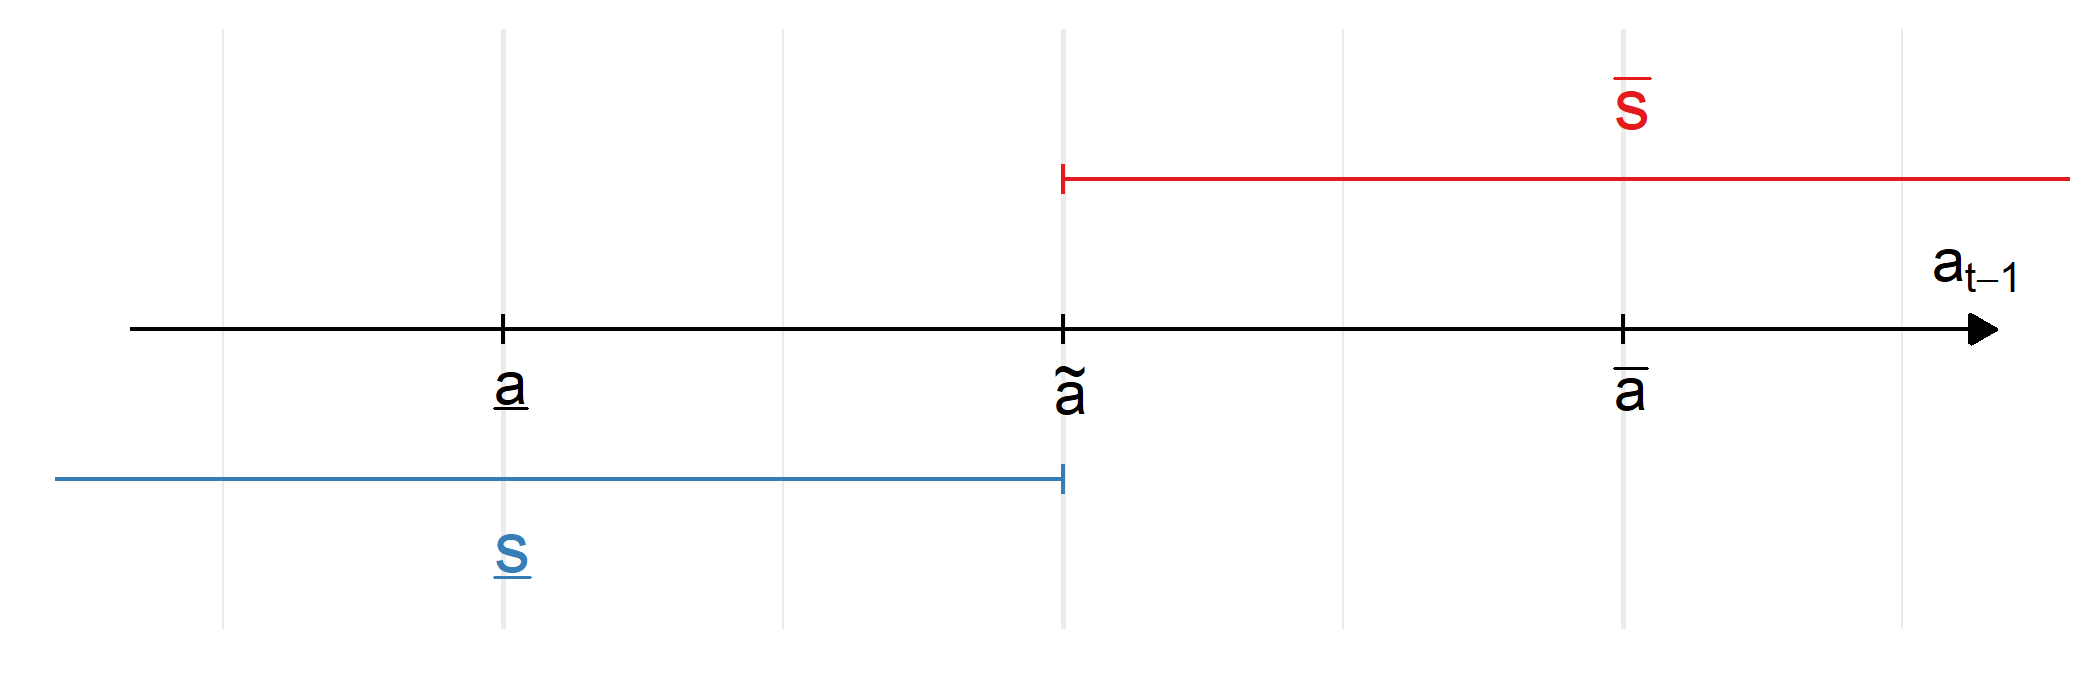
\includegraphics[width=.8\linewidth]{chap3/graphic/theory-choice-a.png}
	\vspace{-3em}
	\justify\singlespacing\footnotesize{\textit{Notes:} This figure presents the indifference value $\widetilde{a}_{t-1}$ which is defined as the threshold value $a$ in $t-1$ such that the agent is indifferent between both groups. In the single-value model, it corresponds to the midpoint value $\widehat{a}$, which is the middle of the distance between the average values in both groups. When the value $a$ in previous period is lower (resp. higher) than the indifference value, the agent prefers to identify with the group $\underline{s}$ (resp. $\overline{s}$).}
\end{figure}
In the single-value model, as long as the value in previous period $a_{t-1}$ is greater (resp. smaller) than the midpoint value $\widehat{a}$, the agent prefers to belong to group $\overline{s}$ (resp. $\underline{s}$). In absence of shocks on her value, the agent converges toward a steady-state value which corresponds to the average value within her group, and the dynamics is given by equation \eqref{chap3-eq:dyn-1val}. What happens when there is a shock?


If an information shock is sufficiently large, the agent identifies with the other group.\footnote{Based on constructivist psychology, a shock on values consists of an event that brings new information to the agent through an experience (\citealt{Levitt2004Transformational}). This latter challenges the agent by questioning her sense of independence, her emotions, her self-awareness, hence, all her perceptions of the meaning of life (i.e. values).} Suppose the agent belongs to the group $\underline{s}$ and she is in her steady state which means that $a_{t-1} = \underline{a}$. There is a shock $\Delta a_{t-1}$ at the end of the period such that her value becomes $a_{t-1}^\prime = a_{t-1} + \Delta a_{t-1}$. Thus, it is straightforward that the agent prefers to keep with her current group $\underline{s}$ as long as the shock does not push $a_{t-1}^\prime$ beyond the threshold---characterized by the indifference value $\widetilde{a}$. Otherwise, the agent prefers to identify with the other group $\overline{s}$. This result leads to Proposition \ref{chap3-prp:shock}. Proof in appendix \ref{chap3-model}.
\begin{proposition}[Shock existence]\label{chap3-prp:shock}
    For any individual, it always exists an information shock such that she prefers to identify with the other group.
\end{proposition}

%%%%% RESULT 1 %%%%%
The single-value model delivers two main results. First, any individual converges to the average value within her group. The length of time to convergence depends on two components: the rate of convergence and the distance with the group-average value. 
On the one hand, the greater is the ratio $\eta_a/\phi_a$, the more costly is the time inconsistency with respect to the group dissonance, hence, the faster the convergence. 
On the other hand, the further the current value is from the group-average value, the slower the convergence.

%%%%% RESULT 2 %%%%%
Second, it is always possible to find a shock such that an individual starts to identify with the other group. The shock requires two conditions to be satisfied: its direction has to be toward the other-group average value and the magnitude has to be sufficiently large. The magnitude depends on the distance between both groups in terms of value and the current value of the individual. The larger is the distance, the greater has to be the shock. When the current value is in a steady state, the magnitude corresponds to the midpoint distance. Otherwise, the closer she is from the midpoint value, the smaller has to be the shock.

\subsection{Two-value model}

We aim to understand the difference in terms of values dynamics when there are two values instead of one. Suppose there are two (motivational types of) values $V_t = (a_t, b_t)\in\mathbb{R}^2$. Consider the same utility function as before but including the second value $b_t$. The maximization program of the agent becomes:
\begin{equation}\label{chap3-eq:maxU-2val}
    \begin{split}
        \max_{a_t, b_t, s_t} U_t(a_t, b_t, s_t) = &-\eta_a\frac{\left[a_t-a_{t-1}\right]^2}{2} -\phi_a\frac{\left[a_t-a^\star(s_t)\right]^2}{2}\\
        &-\eta_b\frac{\left[b_t-b_{t-1}\right]^2}{2} -\phi_b\frac{\left[b_t-b^\star(s_t)\right]^2}{2},
    \end{split}
\end{equation}
where $v^\star(s_t) = \{\underline{v}, \overline{v}\}$ is the average-group value $v\in\{a,b\}$ and $(\eta_a, \phi_a, \eta_b, \phi_b)\in (\mathbb{R}^\star_{+})^4$ are parameters that account for the relative importance of each utility components. 
%
The agent seeks to avoid the same psychological costs as before, namely, time inconsistency and group dissonance, but on two values instead of one. The optimal values are identical to the single-value model, hence, the weighted average between the past value and the average value within the group:
\begin{align*}
    a_t(s_t) =  \frac{\eta_a a_{t-1} + \phi_a a^\star(s_t)}{\eta_a + \phi_a}, \hspace{2em} \text{and} \hspace{2em}%\label{chap3-eq:foc-1val-a}
    b_t(s_t) =  \frac{\eta_b b_{t-1} + \phi_b b^\star(s_t)}{\eta_b + \phi_b}.%\label{chap3-eq:foc-1val-b}
\end{align*}
Thus, the dynamics of values are also identical to equation \eqref{chap3-eq:dyn-1val} and Proposition \ref{chap3-prp:converge} holds. So far, nothing changes with respect to the single-value model although we add one value.

The difference in this setup arises from the inter-dependence between both values. There exist two groups, $\underline{s}$ and $\overline{s}$, in which the average values are respectively $(\underline{a}, \underline{b})$ and $(\overline{a}, \overline{b})$.
Since values are standardized in the population, it implies that $\underline{v}$ and $\overline{v}$ have opposite signs. 
%
We have set the average value $a$ in both groups such that $\overline{a} > 0 > \underline{a}$.
%
Thus, the inter-dependence between values is captured by the sign of $\overline{b}$ (or equivalently by the sign of $\underline{b}$). If $\overline{b}$ is positive, then both values are positively correlated in the population. Otherwise, they are negatively correlated. 

The inter-dependence between values affects the conditions under which the agent prefers to change her group. To illustrate this, suppose the agent belongs to the group $\underline{s}$ and she is in her steady state such that $a_{t-1}=\underline{a}$ and $b_{t-1} = \underline{b}$.
%
There is an information shock on value $a$ at the end of the period, hence, $a_{t-1}^\prime = \underline{a} + \Delta a_{t-1}$. In period $t$, the agent has to choose whether she wants to stay in her group or change for the other group. Her values depend on this choice. If she decides to stay in her current group, her indirect utility is
\begin{equation}\label{chap3-eq:U1under}
    U_t(\underline{s}) = - \gamma_a \left(\Delta a_{t-1}\right)^2.
\end{equation}
Otherwise, she changes her group and gets the following indirect utility:
\begin{equation}\label{chap3-eq:U1over}
    U_t(\overline{s}) = - \gamma_a \big[\overline{a} - \underline{a}-\Delta a_{t-1}\big]^2
    - \gamma_b \big[\overline{b}-\underline{b}\big]^2,
\end{equation}
where $\gamma_b \equiv \frac{\eta_b\phi_b}{2(\eta_b+\phi_b)}>0$. 

The agent decides to change her group \textit{if and only if} the information shock drives her value $a^\prime_{t-1}$ beyond the indifference threshold $\widetilde{a}$, as depicted in figure \ref{chap3-fig:theory-choice-a}. In this example, the indifference value is derived from equations \eqref{chap3-eq:U1under} and \eqref{chap3-eq:U1over} and corresponds to
\begin{equation}\label{chap3-eq:indiff}
    \widetilde{a} = \widehat{a} + \frac{1}{2\gamma}\frac{\big(\overline{b}-\underline{b}\big)^2}{\overline{a}-\underline{a}},
\end{equation}
where $\gamma \equiv \gamma_a/\gamma_b > 0$ and $\overline{a}-\underline{a} > 0$ by definition.
When both values are orthogonal, i.e. $\overline{b}-\underline{b} = 0$, the indifference value corresponds to the one of the single-value model, namely, $\widehat{a}$.

Figure \ref{chap3-fig:theory-shift-a} presents the indifference value as a function of the degree of inter-dependence between values.
\begin{figure}[!tb]
    \centering
    \caption{Indifference value and inter-dependence between values}
    \label{chap3-fig:theory-shift-a}
    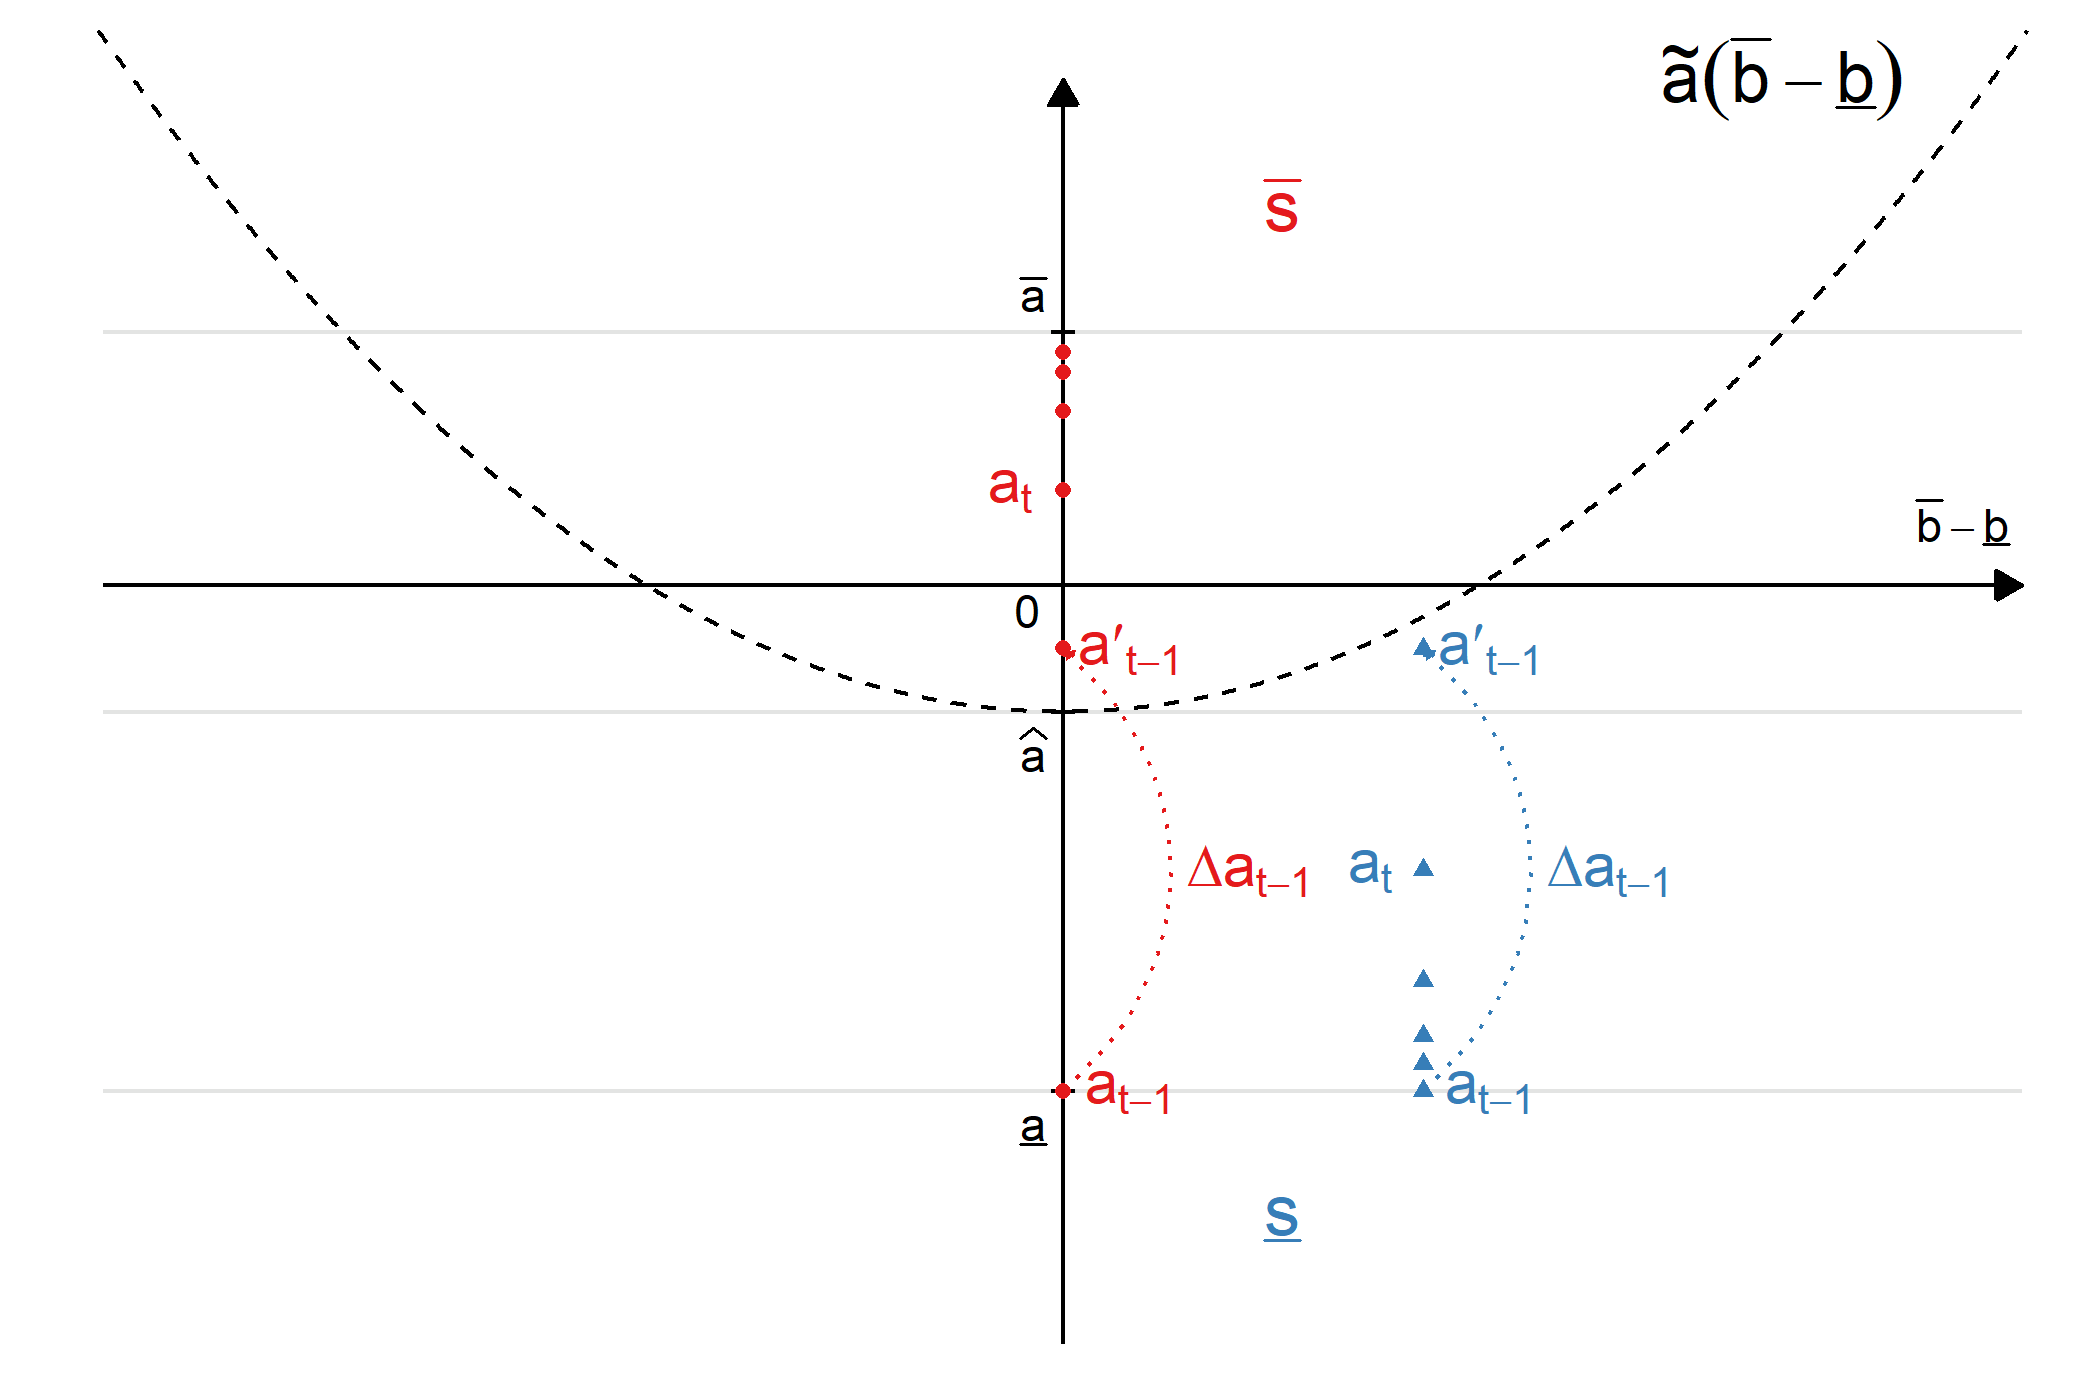
\includegraphics[width=\linewidth]{chap3/graphic/theory-shift-a.png}
	\vspace{-3em}
	\justify\singlespacing\footnotesize{\textit{Notes:} This figure presents the indifference value as a function of the degree of inter-dependence between values. The x-axis corresponds to the gap between both group averages in terms of value $b$. As $\overline{a}-\underline{a} > 0$, it implies that the magnitude of $\overline{b}-\underline{b}$ corresponds to the degree of inter-dependence---values are either positively correlated on the right-hand side of the figure or negatively correlated on the left-hand side.
	The y-axis corresponds to the value $a$. 
	The dash line refers to the indifference value $\widetilde{a}$ and indicates the frontier of indifference between both groups $\overline{s}$ and $\underline{s}$. The dotted curve shows an information shock $\Delta a_{t-1}$ in two different settings, based on the degree of inter-dependence, which lead to different group memberships.}
\end{figure}
The right-hand side of the figure corresponds to cases in which both values are positively correlated, whereas the left-hand side refers to those in which they are negatively correlated. The dashed line represents the indifference value $\widetilde{a}$, which is a function of the distance between both group-average values in $b$, hence, the inter-dependency.

Starting with the area below the dashed curve, any information shock that shifts the value $a$ in this area is not sufficiently large to change the agent's group membership. Thus, agent's value $a$ converges back to its steady-state value $\underline{a}$, and value $b$ has not changed meanwhile.
Conversely, any information shock that brings the value $a$ above the indifference value implies a change in the group membership of the agent. As the agent identifies with the other group, she changes both of her values. In the long run, she converges toward the average values of the other group, namely, $\overline{a}$ and $\overline{b}$. Although the value $b$ was not initially affected by the information shock, the agent has changed her value $b$ to be consistent with the values in her new group. Thus, the two-value model provides a theoretical framework for the existence of spillover effects that is based on group consistency.

Proposition \ref{chap3-prp:shock} holds when there is an additional inter-dependent value, meaning that it is always possible to find a shock sufficiently large such that she prefers to identify with the other group.
Nonetheless, it leads to Proposition \ref{chap3-prp:relevant}.%
\begin{proposition}[Value relevance]\label{chap3-prp:relevant}
    If a value poorly discriminates groups with respect to the other, then this value is less relevant in the individual's choice of group membership.
\end{proposition}%
% % How?
When the gap between groups in terms of value $b$ is large in absolute terms, i.e. $\left|\overline{b}-\underline{b}\right| \gg \overline{a}-\underline{a}$, it indicates that the polarization between both groups in terms of $b$ is important with respect to the one in terms of $a$. Thus, the value $a$ is less relevant for values dynamics as only a very large shock on $a$ can make the agent identify with the other group. This is due to the fact that the group dissonance with respect to $b$ generates a psychological cost that can hardly be offset by any other consideration than keeping up with the current group---except with a large information shock.

\subsection{Predictions of the model}

The theoretical framework provides several predictions about the dynamics of values. 
Proposition \ref{chap3-prp:converge} indicates that, in absence of information shocks, any individual converges in values toward the values of her group.
Proposition \ref{chap3-prp:shock} predicts that, for any individual, it is always possible to find an information shock such that the agent identifies with the other group. The corollary implies that there exist small shocks for which the individual is only affected in the short run as she does not change group.
Both previous predictions hold when the individual is characterized by two values that are correlated across groups, hence, inter-dependent.
Proposition \ref{chap3-prp:relevant} predicts that values that discriminate the most between groups are those that are the most relevant in the choice of the individual about group membership.

The theoretical framework also raises an important issue about considering only one value at a time. The consistency trade-off in individual's group membership depends on the degree of inter-dependence between values across groups. As a result, neglecting this inter-dependence leads to underestimating the role of the group in values dynamics. Thus, the greater the correlation of values across groups, the larger has the shock to be for the agent to change group.

Lastly, Proposition \ref{chap3-prp:spillover} gives the main prediction of the theoretical framework about the existence of spillover effects across values.
\begin{proposition}[Spillover effect]\label{chap3-prp:spillover}
    If two values are inter-dependent, then an information shock on one value can trigger a spillover effect on the other value.
\end{proposition}
When an information shock---due to a life-changing event---on one value is sufficiently large, the individual identifies with another group, thus, she changes both of her values. Although the other value was not initially affected, the life-changing event has also changed this value indirectly through the spillover effect. I turn to empirical analysis in order to test the existence of spillover effects among values.